%=========================================================
% Peripheral : Interrupt Generator (INT_GEN)
%=========================================================
\section{Peripheral : Peripheral : Interrupt Generator (INT\_GEN)}

\begin{description}

    \item[Overview]\mbox{}\\
        INT\_GEN (Interrupt Generator) generates interrupt requests of IRQ\_EXT and IRQ[63:0] by software setting.
        
    \item[Input / Output Signals]\mbox{}\\
        Input / Output signals of INT\_GEN are shown in Table \ref{tb:IOSIGNALS_INTGEN}.


%-------------------------------
\begin{table}[H]
    \begin{adjustbox}{scale={0.65}{0.8}}
    \textsf{
    \begin{tabular}{|L{4cm}{2cm}{t}|L{4cm}{2cm}{t}|L{2cm}{1cm}{t}|L{7cm}{6cm}{t}|L{10cm}{6cm}{t}|L{3cm}{2cm}{t}|}
        \hline
        %-------------------------------------
        \rowcolor{LightPurple}
        \textbf{Group} &
        \textbf{Direction} &
        \textbf{Width} &
        \textbf{Name} &
        \textbf{Description} &
        \textbf{Note}
        \nextRow \hline
        %-------------------------------------
        System & input  & ~ & RES & Reset & ~
        \nextRow \hline
        %-------------------------------------
        System & input  & ~ & CLK & System Clock & ~
        \nextRow \hline
        %-------------------------------------
        AHB    & input  & ~                   & S\_HSEL      & AHB Lite Slave Select & ignored
        \nextRow \hline
        %-------------------------------------
        AHB    & input  & \lbrack  1:0\rbrack & S\_HTRANS    & AHB Lite Slave Transfer Type & ~
        \nextRow \hline
        %-------------------------------------
        AHB    & input  & ~                   & S\_HWRITE    & AHB Lite Slave Write & ~
        \nextRow \hline
        %-------------------------------------
        AHB    & input  &                     & S\_HMASTLOCK & AHB Lite Slave Locked Transfer & ignored
        \nextRow \hline
        %-------------------------------------
        AHB    & input  & \lbrack  2:0\rbrack & S\_HSIZE     & AHB Lite Slave Access Size & ~
        \nextRow \hline
        %-------------------------------------
        AHB    & input  & \lbrack  2:0\rbrack & S\_HBURST    & AHB Lite Slave Burst Access & ignored
        \nextRow \hline
        %-------------------------------------
        AHB    & input  & \lbrack  3:0\rbrack & S\_HPROT     & AHB Lite Slave Protection & ignored
        \nextRow \hline
        %-------------------------------------
        AHB    & input  & \lbrack 31:0\rbrack & S\_HADDR     & AHB Lite Slave Address & ~
        \nextRow \hline
        %-------------------------------------
        AHB    & input  & \lbrack 31:0\rbrack & S\_HWDATA    & AHB Lite Slave Write Data & ~
        \nextRow \hline
        %-------------------------------------
        AHB    & input  & ~                   & S\_HREADY    & AHB Lite Slave Ready Input & ~
        \nextRow \hline
        %-------------------------------------
        AHB    & output & ~                   & S\_HREADYOUT & AHB Lite Slave Ready Output & ~
        \nextRow \hline
        %-------------------------------------
        AHB    & output & \lbrack 31:0\rbrack & S\_HRDATA    & AHB Lite Slave Read Data & ~
        \nextRow \hline
        %-------------------------------------
        AHB    & output & ~                   & S\_HRESP     & AHB Lite Slave Response & always output 0
        \nextRow \hline
        %-------------------------------------
        INT	   & output & ~                   & IRQ\_EXT     & External Interrupt Request & ~
        \nextRow \hline
        %-------------------------------------
        INT    & output & \lbrack 63:0\rbrack & IRQ          & Interrupt Request & ~
        \nextRow \hline
        %-------------------------------------
    \end{tabular}
    }
    \end{adjustbox}
    \caption{Input / Output Signals of INT\_GEN)}
    \label{tb:IOSIGNALS_INTGEN}
\end{table}
%-------------------------------

    \item[Control Registers]\mbox{}\\
        Controls registers of INT\_GEN are shown in Table \ref{tb:REG_IRQEXT}, Table \ref{tb:REG_IRQ0} and Table \ref{tb:REG_IRQ1}, respectively. The interrupt request levels of IRQ\_EXT and IRQ[63:0] are controlled by corresponding bits in each register.
 
\end{description}

%-------------------------------
\begin{table}[H]
    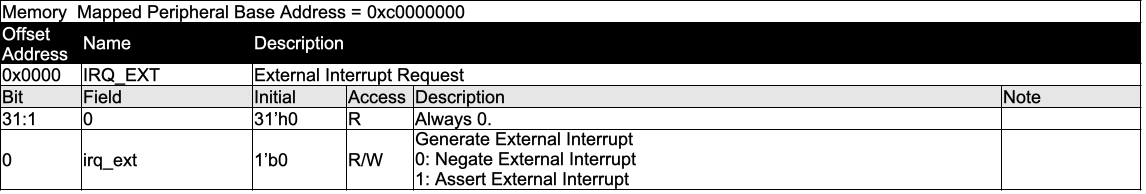
\includegraphics[width=1.0\columnwidth]{./Table/REG_IRQEXT.png}
    \caption{INT\_GEN Control Register IRQ\_EXT)}
    \label{tb:REG_IRQEXT}
\end{table}
%-------------------------------
%-------------------------------
\begin{table}[H]
    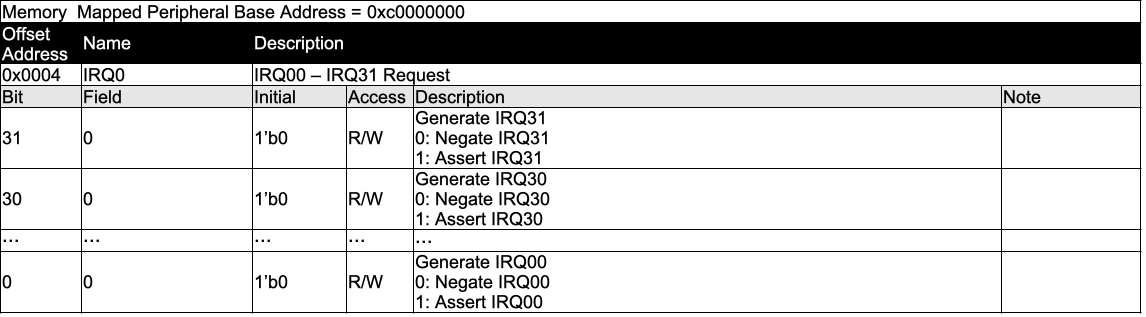
\includegraphics[width=1.0\columnwidth]{./Table/REG_IRQ0.png}
    \caption{INT\_GEN Control Register IRQ0)}
    \label{tb:REG_IRQ0}
\end{table}
%-------------------------------
%-------------------------------
\begin{table}[H]
    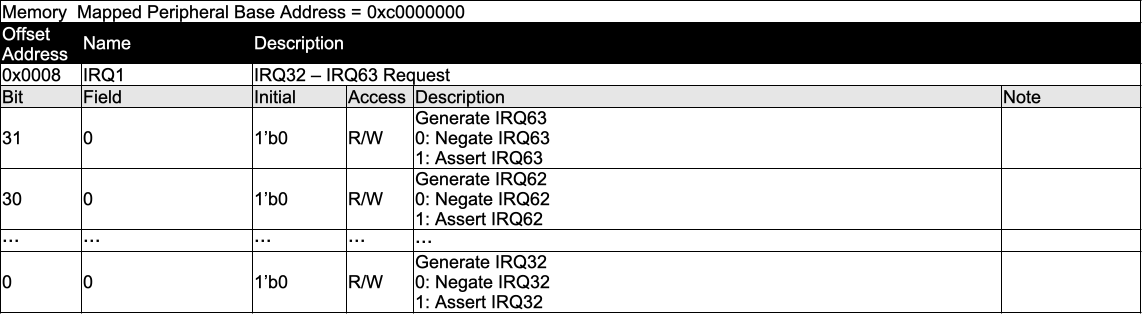
\includegraphics[width=1.0\columnwidth]{./Table/REG_IRQ1.png}
    \caption{INT\_GEN Control Register IRQ1)}
    \label{tb:REG_IRQ1}
\end{table}
%-------------------------------

